\documentclass[acmsmall]{acmart}

% Remove ACM copyright/journal footers
\settopmatter{printacmref=false} % Removes citation info below abstract
\renewcommand\footnotetextcopyrightpermission[1]{} % Removes copyright
\pagestyle{plain} % Removes running headers

\usepackage{subcaption}
\usepackage{float}

\begin{document}

\title{Comparative Analysis of Hashing, Bloom Filters, and Cuckoo Filters for Membership Testing}

\author{Aarav Gosalia}
\affiliation{%
  \institution{University of British Columbia Okanagan}
  \city{Kelowna}
  \country{Canada}}

\begin{abstract}
Membership testing is a fundamental problem in computer science and data processing, where the task is to decide whether a given element (e.g., a username, a word, or a network address) is part of a stored set.

This report presents a comparison of different techniques: linear and binary search (baseline exact methods), hashing (exact membership), Bloom filters (probabilistic with false positives), and Cuckoo filters (probabilistic with deletions and potential false negatives). I generate large-scale synthetic datasets, run benchmarks across dataset sizes ($10K$, $100K$, $1M$, $10M$, $100M$), and analyze runtime and accuracy trade-offs. Due to computational and storage constraints, only smaller datasets are stored in the GitHub repository, while large-scale tests are reported but excluded from version control. 
\end{abstract}

\keywords{Hashing, Bloom Filter, Cuckoo Filter, Membership Testing, Probabilistic Data Structures}

\maketitle

\section{Introduction}
Membership testing is the task of determining whether a particular element exists within a set. It is a core operation in computer science, with applications ranging from login username checking and spell checking to intrusion detection and large-scale web systems. As datasets grow, the efficiency and scalability of membership tests become critical.  

This assignment focuses on comparing several techniques for membership testing. I begin with two baseline approaches: \textbf{linear search}, which checks elements one by one, 
and \textbf{binary search}, which operates on sorted data. Both are exact but can become slow at scale. I then study more advanced techniques: \textbf{hashing}, which provides expected constant-time lookups, and two probabilistic data structures, the \textbf{Bloom filter} and the \textbf{Cuckoo filter}.  

The goal of this work is to benchmark these methods in terms of runtime, accuracy, and error rates, using synthetic datasets of increasing sizes. By comparing exact and probabilistic approaches, I highlight the trade-offs between speed, memory  usage, and correctness.

\section{Background}
This section describes the membership testing techniques considered in this study, their underlying data structures, and their theoretical performance.

\subsection{Linear Search}
Linear search is the simplest approach: given a query, each element of the dataset is checked sequentially. This requires no preprocessing or additional data structures.  
\begin{itemize}
  \item Time complexity: $O(n)$ per query.  
  \item Space complexity: $O(n)$ to store the list of elements.  
\end{itemize}
Although easy to implement, linear search is impractical for large datasets, which is why in this study I restricted it to datasets of up to $1M$ elements.

\subsection{Binary Search}
Binary search improves efficiency by operating on sorted data. It repeatedly halves the search interval until the query is found or the interval is empty.  
\begin{itemize}
  \item Time complexity: $O(\log n)$ per query (after an $O(n \log n)$ sort).  
  \item Space complexity: $O(n)$ storing the sorted list.  
\end{itemize}
Binary search is much faster than linear search, but requires sorting in advance and is still slower than hashing or probabilistic methods for large-scale queries.

\subsection{Hashing}
Hashing uses a hash table or set data structure. Each element is mapped to a bucket using a hash function, allowing for near-constant time lookups. In our implementation, Python’s built-in \texttt{set()} was used, which internally maintains a hash table with dynamic resizing and open addressing.  
\begin{itemize}
  \item Time complexity: $O(1)$ average case, $O(n)$ worst case.  
  \item Space complexity: $O(n)$, but with overhead due to hash buckets and pointers (larger than sorted arrays).  
\end{itemize}
Hashing provides exact results, unlike probabilistic methods, but can consume more memory. Compared to binary search, it is usually faster but less cache-friendly.

\subsection{Bloom Filter}
A Bloom filter is a probabilistic structure that uses a fixed-size bit array and multiple independent hash functions. When inserting an element, each hash function computes an index and marks the corresponding bit in the array. To test membership, 
all of those bits are checked:  
\begin{enumerate}
  \item If any of the bits is 0, the element is \emph{definitely not present}.  
  \item If all are 1, the element is \emph{possibly present}.  
\end{enumerate}

\begin{itemize}
  \item Time complexity: $O(k)$ per query/insert, where $k$ is the number of hash functions (usually small, e.g., 3–7).  
  \item Space complexity: $O(n \log (1/\epsilon))$ bits, where $\epsilon$ is the target false positive probability. This is significantly smaller than storing all elements explicitly.  
  \item Error: False positives are possible; false negatives are impossible.  
\end{itemize}

In this project I used the \texttt{pybloom-live} Python package \cite{pybloom}, which provides a standard implementation of Bloom filters. Compared to hashing, Bloom filters save memory by not storing the elements themselves. They are especially useful when the dataset is very large and only approximate membership is acceptable.

\subsection{Cuckoo Filter}
Cuckoo filters are based on the idea of \emph{Cuckoo hashing}. Instead of storing full elements, they store short \emph{fingerprints} (a few bits) of each element inside hash table ``buckets.'' Each element can be placed in one of two possible buckets determined by its hash. If both are full, an existing fingerprint is ''kicked out'' (cuckoo-style) and reinserted into its alternate location. This process may cascade, 
but typically completes quickly.

To check membership, the query’s fingerprint is computed and checked against both possible buckets.  

\begin{itemize}
  \item Time complexity: $O(1)$ expected per query/insert, similar to Bloom filters.  
  \item Space complexity: $O(n \cdot f)$ bits, where $f$ is the fingerprint size (commonly 4–8). In practice this is lower than hashing (since only fingerprints are stored), but typically higher than Bloom filters (due to bucket structures and relocation).  
  \item Error: False positives are possible; false negatives are rare under very high load or after repeated insertions and relocations if items are dropped.  
\end{itemize}

Compared to Bloom filters, Cuckoo filters have two major advantages:
\begin{enumerate}
  \item They support \textbf{deletion} of elements, since fingerprints can be removed from buckets (something Bloom filters cannot do without extensions).  
  \item They avoid the fixed $k$ hash lookups of Bloom filters — instead, only two buckets are checked.  
\end{enumerate}

In this project, I used the \texttt{cuckoopy} Python package \cite{cuckoopy}, which provides a practical implementation of Cuckoo filters with tunable parameters (bucket size, fingerprint length).  

\section{Methodology}
I implemented each membership method in Python and tested them using synthetic datasets.  

\subsection{Dataset Generation}
Two types of files were used:  
\begin{itemize}
  \item \texttt{logins\_N.csv}: containing randomly generated usernames representing the stored dataset, where $N \in \{10K, 100K, 1M, 10M, 100M\}$.  
  \item \texttt{queries\_Q.csv}: containing query usernames along with a label (\texttt{is\_present}) indicating whether they truly belong to the dataset. $Q$ was set to about $10\%$ of $N$.  
\end{itemize}

The usernames were created using synthesized functions: sequential (\texttt{user0}, \texttt{user1}, ...), adjective-noun combinations (\texttt{brave\_otter\_15}), and random-looking strings with indices. A mixed scheme randomly selected among these, producing a varied dataset. Queries were generated with a controlled \emph{duplication rate} (50\% present, 50\% absent).  

Large files (\texttt{logins\_10M.csv}, \texttt{logins\_100M.csv}, and corresponding queries) were too large to upload to GitHub (exceeding size limits) and were excluded via \texttt{.gitignore}. Smaller datasets were retained for reproducibility.  

\subsection{Evaluation Procedure}
Each method was implemented as a function that:  
\begin{enumerate}
  \item Loaded the dataset of logins.  
  \item Iterated over the query set.  
  \item Checked membership using the corresponding data structure.  
  \item Recorded true positives, true negatives, false positives, and false negatives.  
\end{enumerate}

For hashing, Python’s built-in \texttt{set()} was used. For Bloom filters, the \texttt{pybloom-live} package was used with error rate 0.001. For Cuckoo filters, the \texttt{cuckoopy} package was used with bucket size 2 and fingerprint length 4 bits.  

\subsection{Benchmarking}
For each dataset size ($10K$, $100K$, $1M$, $10M$, $100M$):  
\begin{itemize}
  \item I measured \textbf{runtime} for all queries.  
  \item I calculated \textbf{accuracy} as $(TP+TN)/(TP+TN+FP+FN)$.  
  \item I reported \textbf{false positive rates} for Bloom and Cuckoo filters.  
\end{itemize}
Linear search was only applied to $N \leq 1M$, since beyond that the runtime would be prohibitively long on the available hardware (Apple MacBook Pro M2). The Cuckoo filter was also skipped at $N=100M$, as it consumed excessive memory and took too long to run on this machine. Similarly, I did not attempt to generate a dataset of size $N=1B$, as the time and memory required would exceed practical limits. 

\section{Results}

This section presents the experimental outcomes of benchmarking the five membership testing methods (Linear, Binary, Hash, Bloom, Cuckoo). I report runtimes, accuracies, and error counts across dataset sizes ranging from 10K to 100M.  

\subsection{Runtime Plots}

Figure~\ref{fig:linear-runtime} shows the runtime of linear search on smaller datasets only (10K, 100K, 1M). Figure~\ref{fig:other-runtime} compares Binary, Hash, Bloom, and Cuckoo across all dataset sizes. As discussed, Cuckoo at 100M was skipped due to excessive memory use and runtime overhead.

\begin{figure}[H]
    \centering
    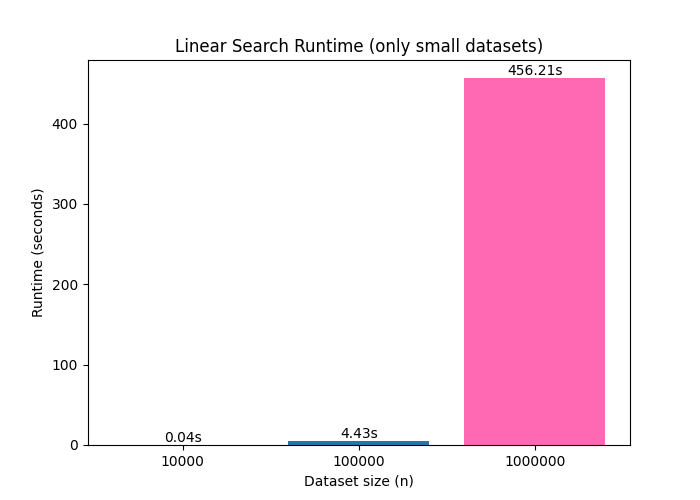
\includegraphics[width=0.7\linewidth]{plots/linear_plot.png}
    \caption{Runtime of Linear Search on smaller datasets (10K, 100K, 1M).}
    \label{fig:linear-runtime}
\end{figure}

\begin{figure}[H]
    \centering
    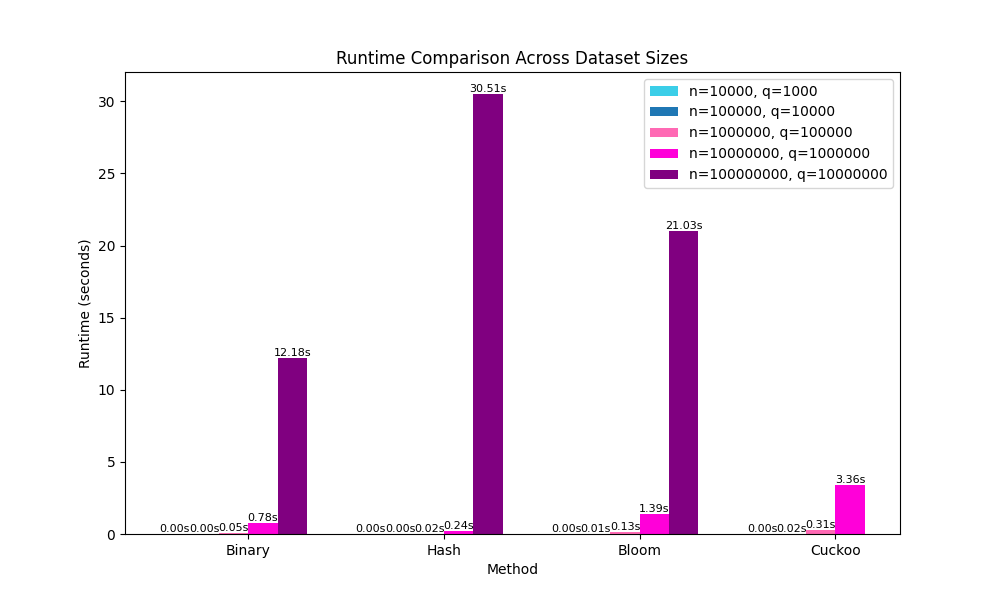
\includegraphics[width=0.8\linewidth]{plots/other_plot.png}
    \caption{Runtime comparison of Binary, Hash, Bloom, and Cuckoo filters across all dataset sizes.}
    \label{fig:other-runtime}
\end{figure}

\subsection{Detailed Results Tables}

Tables~\ref{tab:results-small} and \ref{tab:results-large} summarize runtimes, accuracies, false positives (FP), and false negatives (FN). For compactness, the first three dataset sizes (10K, 100K, 1M) are shown side by side, and the last two (10M, 100M) are shown below.

% ---------------- SMALL TABLES (2 per row) ----------------
\begin{table}[h]
\centering
\caption{Results for smaller datasets (10K, 100K, 1M).}
\label{tab:results-small}
\begin{tabular}{cc}
\begin{minipage}{0.45\linewidth}
\centering
\subcaption{10K (q=1K)}\label{tab:results-10k}
\begin{tabular}{lcccc}
\toprule
Method & Time & Acc. & FP & FN \\
\midrule
Linear & 0.0450 & 1.0000 & 0 & 0 \\
Binary & 0.0002 & 1.0000 & 0 & 0 \\
Hash   & 0.0001 & 1.0000 & 0 & 0 \\
Bloom  & 0.0011 & 1.0000 & 0 & 0 \\
Cuckoo & 0.0021 & 0.9930 & 0 & 7 \\
\bottomrule
\end{tabular}
\end{minipage}
&
\begin{minipage}{0.45\linewidth}
\centering
\subcaption{100K (q=10K)}\label{tab:results-100k}
\begin{tabular}{lcccc}
\toprule
Method & Time & Acc. & FP & FN \\
\midrule
Linear & 4.4328 & 1.0000 & 0 & 0 \\
Binary & 0.0028 & 1.0000 & 0 & 0 \\
Hash   & 0.0009 & 1.0000 & 0 & 0 \\
Bloom  & 0.0127 & 0.9999 & 1 & 0 \\
Cuckoo & 0.0243 & 0.9960 & 0 & 40 \\
\bottomrule
\end{tabular}
\end{minipage}
\end{tabular}
\end{table}

\begin{table}[h]
\centering
\caption{Results for 1M dataset.}
\label{tab:results-1M}
\begin{tabular}{lcccc}
\toprule
Method & Time & Acc. & FP & FN \\
\midrule
Linear & 456.2058 & 1.0000 & 0 & 0 \\
Binary & 0.0457 & 1.0000 & 0 & 0 \\
Hash   & 0.0172 & 1.0000 & 0 & 0 \\
Bloom  & 0.1292 & 0.9995 & 49 & 0 \\
Cuckoo & 0.3078 & 0.9955 & 0 & 449 \\
\bottomrule
\end{tabular}
\end{table}

% ---------------- LARGE TABLES ----------------
\begin{table}[h]
\centering
\caption{Results for larger datasets (10M, 100M).}
\label{tab:results-large}
\begin{tabular}{cc}
\begin{minipage}{0.45\linewidth}
\centering
\subcaption{10M (q=1M)}\label{tab:results-10M}
\begin{tabular}{lcccc}
\toprule
Method & Time & Acc. & FP & FN \\
\midrule
Binary & 0.7806 & 1.0000 & 0 & 0 \\
Hash   & 0.2404 & 1.0000 & 0 & 0 \\
Bloom  & 1.3908 & 0.9995 & 534 & 0 \\
Cuckoo & 3.3643 & 0.9955 & 0 & 4502 \\
\bottomrule
\end{tabular}
\end{minipage}
&
\begin{minipage}{0.45\linewidth}
\centering
\subcaption{100M (q=10M)}\label{tab:results-100M}
\begin{tabular}{lcccc}
\toprule
Method & Time & Acc. & FP & FN \\
\midrule
Binary & 12.1779 & 1.0000 & 0 & 0 \\
Hash   & 30.5110 & 1.0000 & 0 & 0 \\
Bloom  & 21.0310 & 0.9995 & 5120 & 0 \\
Cuckoo & \multicolumn{4}{c}{Skipped (too large)} \\
\bottomrule
\end{tabular}
\end{minipage}
\end{tabular}
\end{table}

\section{Discussion}
The experimental results clearly illustrate how different membership testing methods behave as dataset sizes increase from 10K to 100M.  

As expected, \textbf{linear search} performed the worst. Its runtime grew rapidly with $n$, becoming completely impractical at 1M (over 450 seconds). The runtime plot in Figure~\ref{fig:linear-runtime} highlights this steep scaling, which is why I restricted linear search to datasets of size 1M or smaller.  

\textbf{Binary search} produced a more surprising outcome. While its logarithmic time complexity is well understood, the benchmarks show that it scaled extremely well in practice and even outperformed all methods except hashing at 10M. This likely stems from the efficiency of Python’s highly optimized sorting and array access, which make repeated binary lookups extremely fast and cache-friendly.  

\textbf{Hashing} (using Python’s \texttt{set()}) delivered excellent performance up to 10M, consistently outperforming binary search. However, at 100M it scaled poorly, taking longer than both binary search and Bloom filters. This may be due to memory management overheads, cache inefficiency at very large sizes, or RAM limitations on the test hardware (MacBook Pro M2). Since Python sets allocate memory dynamically and maintain internal hash buckets, their efficiency can degrade when memory pressure grows.  

The \textbf{Bloom filter} maintained solid performance across all tested dataset sizes. At 100M, it scaled better than hashing, completing in about 21 seconds compared to 30 seconds for hash sets. However, Bloom filters inherently allow false positives. In our tests, this meant that some absent usernames were incorrectly reported as present. This behavior is consistent with Bloom filter theory, where false positives occur due to overlapping bit positions, while false negatives remain impossible.  

The \textbf{Cuckoo filter} also performed well up to 10M, with runtimes in the same ballpark as Bloom. However, it produced false negatives, meaning that some queries for truly present usernames were reported as absent. This issue arises from fingerprint collisions and bucket evictions under high load. For the 100M dataset, the Cuckoo filter was skipped entirely, since it consumed excessive memory and took too long to run on the available hardware.  

Overall, the runtime plot in Figure~\ref{fig:other-runtime} shows a clear story: binary search, hashing, Bloom, and Cuckoo all vastly outperform linear search, but each comes with trade-offs in scaling and correctness. Surprisingly, binary search often outpaced the probabilistic methods, which were expected to dominate at larger scales.

\section{Conclusion}
This study compared linear search, binary search, hashing, Bloom filters, and Cuckoo filters for the task of membership testing. The results highlight several key points:  
\begin{itemize}
  \item Linear search quickly became impractical, confirming its $O(n)$ scaling.  
  \item Binary search performed far better than expected, scaling gracefully and even outperforming Bloom and Cuckoo filters despite being an exact method.  
  \item Hashing showed outstanding performance until 10M, but then scaled poorly at 100M, likely due to memory and caching issues.  
  \item Bloom filters scaled reliably to 100M, but produced false positives as expected.  
  \item Cuckoo filters worked well up to 10M but produced false negatives and could not be tested at 100M due to hardware constraints.  
\end{itemize}

The most surprising result was the strength of binary search, which consistently rivaled or outperformed probabilistic methods that sacrifice accuracy for speed. However, it is important to note the limitations of this study: only moderate dataset sizes (up to 100M) were tested, constrained by the performance of the MacBook Pro M2. For even larger datasets, probabilistic methods such as Bloom and Cuckoo filters may demonstrate their true advantages.  

In conclusion, while binary search emerged as a surprisingly strong competitor, further testing at larger scales and on more powerful hardware is necessary to fully evaluate the benefits of Bloom and Cuckoo filters in real-world applications.

\section*{GitHub Repository}
The full code (dataset generation, benchmark scripts, and unit tests) is available at:  
\url{https://github.com/your-username/your-repo-name}

\section*{Acknowledgements}
This report was partly supported by interactive assistance from ChatGPT \cite{chatgpt}, which was used for code troubleshooting, clarifications, and grammar review.

\bibliographystyle{ACM-Reference-Format}
\bibliography{refs}

\end{document}
